\subsubsection*{Demostraciones}
\providecommand{\abs}[1]{\lvert#1\rvert}
\providecommand{\norm}[1]{\lVert#1\rVert}

1) Justificar que:
\begin{displaymath}
A = p WD + ez^{t}
\end{displaymath}

Estudiemos como son los elementos de la matriz $A = p WD + ez^{t}$:

\begin{displaymath}
(p WD + ez^{t})_{ij} = p(W\,D)_{ij}+(ez^{t})_{ij} = p(\sum_{k=1}^{n}w_{ik}d_{kj}+1\,z^{t}_j)
\end{displaymath}

Como D es una matriz diagonal, los elementos distintos de cero únicamente pueden estar en la diagonal, con lo cual al hacer el producto se anulan todos los términos con $k\not=j$ y también aquellos términos donde $w_{ik}=0$ lo cual ocurre cuando $c_j=0$.

En consecuencia se puede reescribir:

\begin{displaymath}
(p WD + ez^{t})_{ij} = p(w_{ij}d_{jj}+z^{t}_j)
\end{displaymath}

Vamos a separar en casos para analizar los posibles valores que puede tomar el elemento (notar que por la definición de D, la condición $d_{jj}=0$ es equivalente a $c_j=0$):

caso 1: $w_{ij}=0, d_{jj}=0$ ($c_j=0$)$\Rightarrow(p WD + ez^{t})_{ij} =z_j^t=1/n$


caso 2: $w_{ij}=0, d_{jj}\not=0$ ($c_j\not=0$)$\Rightarrow(p WD + ez^{t})_{ij} =z_j^t=(1-p)/n$


caso 3: $w_{ij}=1, d_{jj}=0$ ($c_j=0$)$\Rightarrow(p WD + ez^{t})_{ij} =z_j^t=1/n$


caso 4: $w_{ij}=1, d_{jj}\not=0$ ($c_j\not=0$)$\Rightarrow(p WD + ez^{t})_{ij} =p/c_j+z_j^t=p/c_j+(1-p)/n$

Observando los casos 2 y 4 podemos observar que se pueden  unificar en una condición equivalente: $(p WD + ez^{t})_{ij} =w_{ij}p/c_j+z_j^t=p/c_j+(1-p)/n$

Uniendo todo lo anterior tenemos que:


\begin{equation}
 (p WD + ez^{t})_{ij} = \left\{
    \begin{array}{ll}
	 p\,w_{ij}/c_j+z_j^t=(1-p)/n+p/c_j & \mathrm{si\ } c_j \not= 0 \\
	 1/n & \mathrm{si\ } c_j=0
	 \end{array}
   \right.
\end{equation}
Pero precisamente esto coincide con la definición de los elementos de la matriz A. Luego $A = p WD + ez^{t}$.
%demostracion 2como se garantiza la aplicabilidad de EG

2) ¿Cómo se garantiza la aplicabilidad de la Eliminación Gaussiana? ¿La matriz $I-pWD$ está bien condicionada?¿Cómo influye el valor de p?

Primero veamos como se garantiza la aplicabilidad de Eliminación Gaussiana:

Sea $B=W\,D$,
\begin{displaymath}
B_{ij}=\sum_{k=1}^n w_{ik}d_{kj}
\end{displaymath}

Por la definición de D, cuando $k\not=j$, $d_{kj}=0$, por lo tanto se anulan los correspondientes términos de la sumatoria, quedando:

\begin{displaymath}
B_{ij}=w_{ij}d_{jj}
\end{displaymath}

También sabemos por la definición de W que $w_{jj}=0$ (porque no se consideran los autolinks), así que podemos deducir que los elementos de la diagonal van a ser iguales a cero, luego:

\begin{equation}
 B_{ij} = \left\{
    \begin{array}{ll}
	 0 & \mathrm{si\ } i=j \\
	 1/c_j & \mathrm{si\ } i\not=j,  w_{ij}\not=0
	 \end{array}
   \right.
\end{equation}

Y por lo tanto:

\begin{equation}
(I-p B)_{ij} = \left\{
    \begin{array}{ll}
	 1 & \mathrm{si\ } i=j \\
	 -p/c_j & \mathrm{si\ } i\not=j
	 \end{array}
   \right.
\end{equation}

La matriz B tiene la particularidad de que la suma de los elementos de cada columna es igual a 1, ya que en cada columna hay $c_j$ elementos de valor $1/c_j$. Por lo tanto en $I-p B$ la suma de los elementos de cada columna es $1+c_j\, p/c_j$ con $|c_j\, p/c_j|<1$ porque $0<p<1$. De esto se desprende que $(I-p B)^t$ es estrictamente diagonal dominante y como se probó en la teórica esto implica que sea no singular. Además, si una matriz es e.d.d. cada una de sus submatrices principales es e.d.d. y entonces todas ellas son no singulares. Por otra parte se puede probar que si una matriz tiene inversa, su traspuesta tiene inversa (ejercicio 23 c), Práctica 1). Luego podemos afirmar que $(I-p B)$ es no singular y que todas sus submatrices principales también son no singulares, esto garantiza que $(I-p B)$ tiene descomposición $LU$ que es equivalente a decir que puede realizarse la Eliminación Gaussiana sin necesidad de pivoteo en ninguno de los pasos del proceso.

Con respecto al condicionamiento de la matriz, se puede aplicar una propiedad demostrada en la práctica (ejercicio 21, Práctica 2) la cual afirma que: Dada $M \in$ $\mathbb{R}^{nxn}$ tal que $||M||<1$, $I$ la matriz identidad de $\mathbb{R}^{nxn}$ 
i $||.||$ norma inducida por una norma vectorial: $I+M$ es inversible y $||(I+R)^{-1}||\leq 1/(1-||M||)$.\\

De lo que vimos arriba acerca del formato de las matrices tratadas en el TP, también deducimos que tomando $||.||_1$, $M = -pWD$ estamos en las hipótesis del ejercicio, porque:

\begin{displaymath}
||-pWD||_1=||pWD||_1=|p|||WD||_1=p*c_j*1/c_j=p.
\end{displaymath}
Y como $p<1$, implica que:
\begin{displaymath}
||(I-pWD)^{-1}||_1\leq 1/(1-||I-pWD||_1)
\end{displaymath}
Si calculamos el número de condición,
\begin{displaymath}
K=||I-pWD||||(I-pWD)^{-1}||\leq (1+p) (1/(1-||pWD||)=(1+p) (1/(1-p||WD||)=(1+p)/(1-p)
\end{displaymath}

Cuanto menor sea $p$ mas cerca de 1 estará el número de condición, lo cual es lógico porque la matriz se parecerá más a I que tiene la característica de tener sus columnas ortogonales. A medida que crece $p$ va aumentando el valor de $K$ tendiendo a infinito si $p$ tiende a 1. en el gráfico \ref{K(p)} se puede ver la relación entre el número de condición y el valor de $p$. Con un ejemplo se puede ver que con un valor relativamente cercano a 1 (0.9) el número de condición sigue siendo aceptable, y recién con valores mayores se puede decir que aumenta rápidamente.
Supongamos p = 0.9:
$K\leq (1.9/0.1)=19$.

Para p=0.99: 
$K\leq (1.99/0.01)=199$. 

\begin{figure}[H]
  \centering
    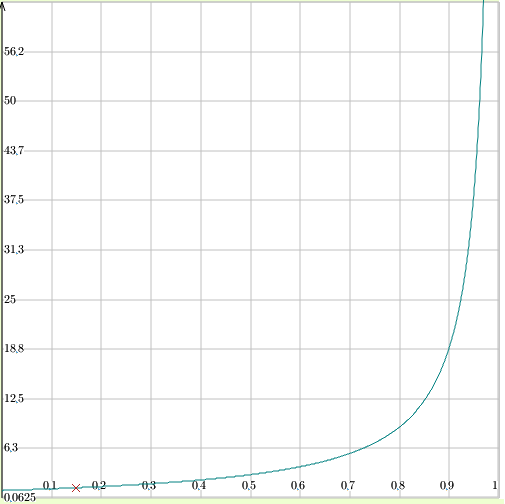
\includegraphics[width=0.7\textwidth]{img/K_tp1.png}
  \caption{K en función de p}
  \label{fig:K(p)}
\end{figure}


\subsubsection*{Tests Cualitativos}



\begin{figure}[H]
  \centering
    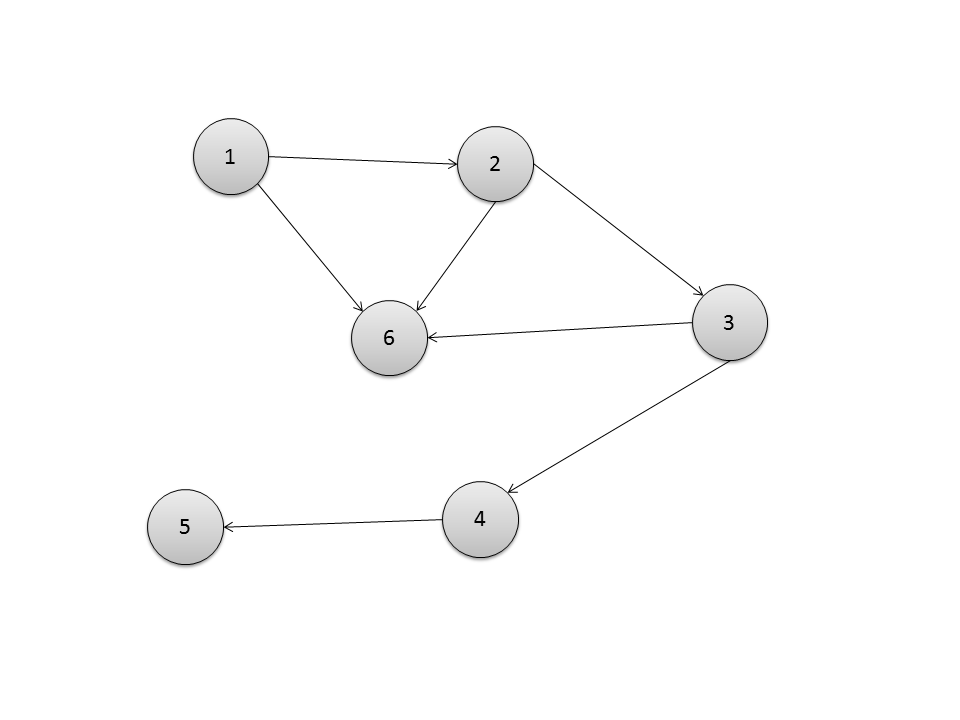
\includegraphics[width=0.7\textwidth]{img/Cadena6v1.png}
  \caption{Cadena con nodo central (caso 1)}
  \label{fig: Cadena con nodo central (caso 1)}
\end{figure}


\begin{figure}[H]
  \centering
    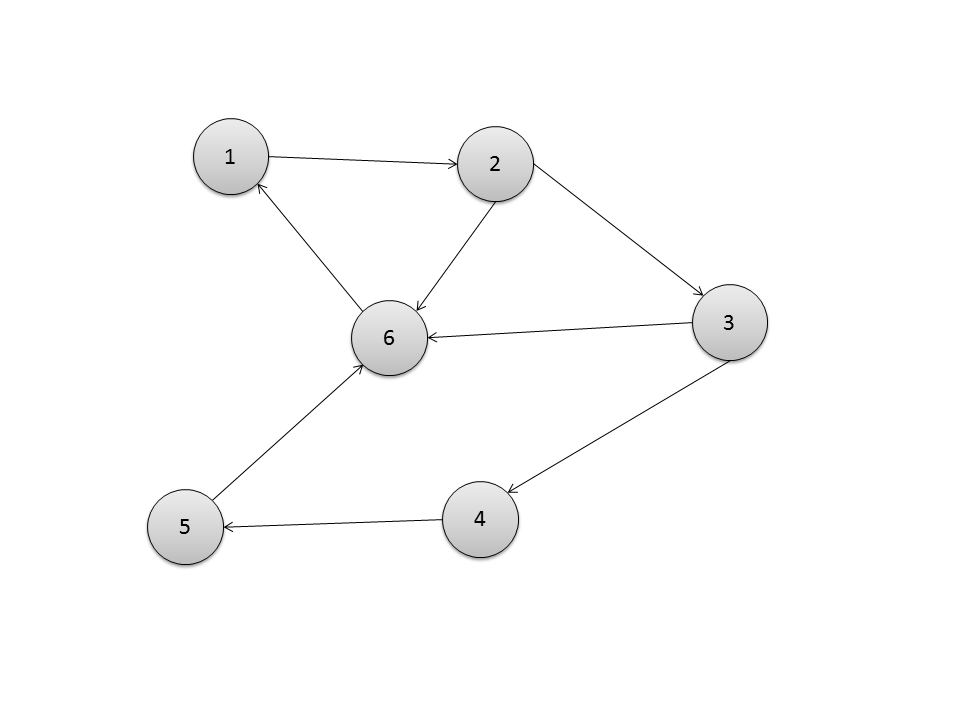
\includegraphics[width=0.7\textwidth]{img/Cadena6v3.png}
  \caption{Cadena con nodo central (caso 3)}
  \label{fig: Cadena con nodo central, con ciclo}
\end{figure}


\begin{figure}[H]
  \centering
    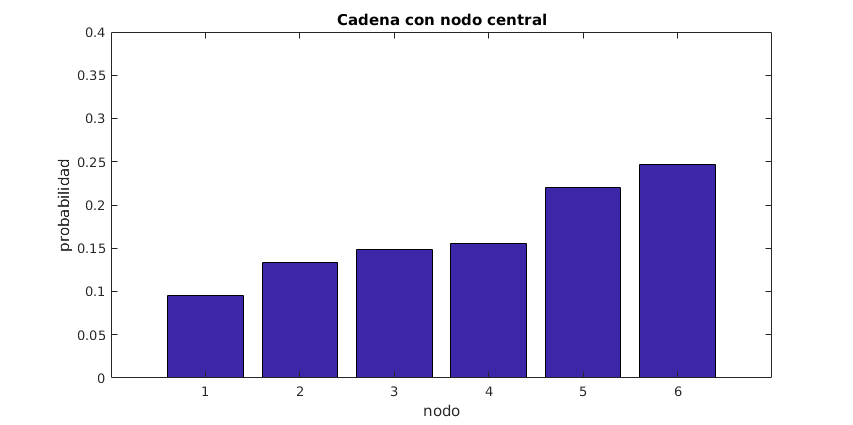
\includegraphics[width=0.7\textwidth]{img/cadena6v1.png}
  \caption{Cadena con nodo central (caso 1)}
  \label{fig: Cadena con nodo central (caso 1)}
\end{figure}


\begin{figure}[H]
  \centering
    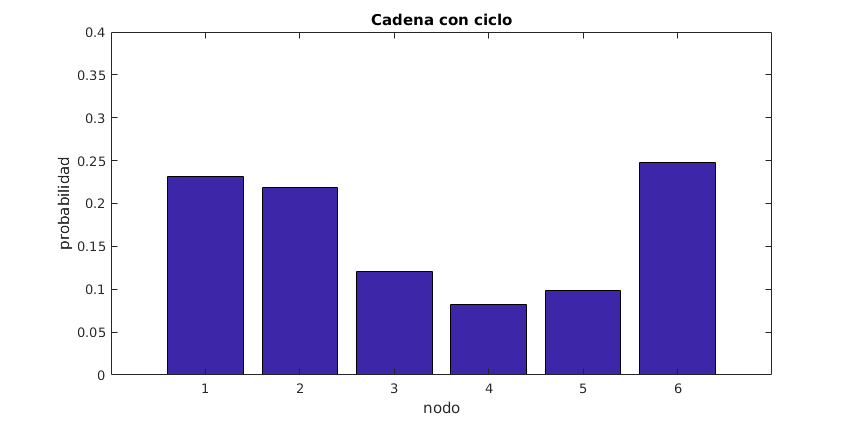
\includegraphics[width=0.7\textwidth]{img/cadena6v3.png}
  \caption{Cadena con nodo central (caso 3)}
  \label{fig: Cadena con nodo central, con ciclo}
\end{figure}

\begin{table}[H]
\centering
	\begin{tabular}{|c|c|c|c|}
		\hline
		Nodo & Probabilidad & Nodo & Probabilidad \\ \hline
		4    & 0.092437     & 1    & 0.0372149    \\
		24   & 0.0815273    & 5    & 0.0372149    \\
		14   & 0.0768427    & 6    & 0.0117647    \\
		18   & 0.0677026    & 7    & 0.0117647    \\
		21   & 0.0650155    & 8    & 0.0117647    \\
		12   & 0.0640465    & 9    & 0.0117647    \\
		2    & 0.0636255    & 10   & 0.0117647    \\
		3    & 0.0636255    & 11   & 0.0117647    \\
		17   & 0.0630019    & 15   & 0.0117647    \\
		23   & 0.0443756    & 16   & 0.0117647    \\
		25   & 0.0443756    & 20   & 0.0117647    \\
		13   & 0.0425018    & 22   & 0.0117647    \\
		19   & 0.0388457    & ~    & ~            \\ \hline
	\end{tabular}
\caption {Tabla de resultados}
\end{table}

\begin{table}[H]
\centering
	\begin{tabular}{|c|c|c|c|}
		\hline
		Nodo & Probabilidad & Nodo & Probabilidad \\ \hline
		2    & 0.155359     & 19   & 0.0150538    \\
		1    & 0.13504      & 21   & 0.0136201    \\
		8    & 0.122903     & 4    & 0.0107527    \\
		6    & 0.118784     & 5    & 0.0107527    \\
		13   & 0.0819211    & 9    & 0.0107527    \\
		3    & 0.0599138    & 10   & 0.0107527    \\
		7    & 0.0582664    & 11   & 0.0107527    \\
		18   & 0.0347814    & 20   & 0.0107527    \\
		17   & 0.0255484    & 22   & 0.0107527    \\
		14   & 0.0227957    & 23   & 0.0107527    \\
		12   & 0.017233     & 24   & 0.0107527    \\
		16   & 0.0162007    & 25   & 0.0107527    \\
		15   & 0.0150538    & ~    & ~            \\ \hline
	\end{tabular}
\caption{Tabla de resultados links a ciclo}
\end{table}

\begin{table}[H]
\centering
	\begin{tabular}{|c|c|c|c|}
		\hline
		Nodo & Probabilidad & Nodo & Probabilidad \\ \hline
		22   & 0.0795721    & 12   & 0.0262073    \\
		2    & 0.0783998    & 17   & 0.0262073    \\
		1    & 0.0764254    & 18   & 0.0262073    \\
		6    & 0.0739574    & 19   & 0.0242481    \\
		20   & 0.0717109    & 4    & 0.0172595    \\
		8    & 0.068699     & 5    & 0.0172595    \\
		21   & 0.0604193    & 9    & 0.0172595    \\
		16   & 0.0452139    & 10   & 0.0172595    \\
		7    & 0.0447391    & 11   & 0.0172595    \\
		13   & 0.0447391    & 23   & 0.0172595    \\
		15   & 0.0438162    & 24   & 0.0172595    \\
		3    & 0.0381661    & 25   & 0.0172595    \\
		14   & 0.0331959    & ~    & ~            \\ \hline
	\end{tabular}
\caption{Tabla de resultados links a ciclo al reves}
\end{table}


\section{Referencias}
\begin{thebibliography}{9}

\bibitem{navegante} 

http://www-2.dc.uba.ar/materias/metnum/dnload/2018\_C1/tp1/Enunciado\_TP1.pdf

\bibitem{burden} 
Richard L. Burden, J. Douglas Faires
\textit{Numerical Analysis}. (Ingles) 
[\textit{An\'alisis num\'erico}]. 
International Thomson, :358-362, 9th Edition, 2010.

\end{thebibliography}


\newpage
%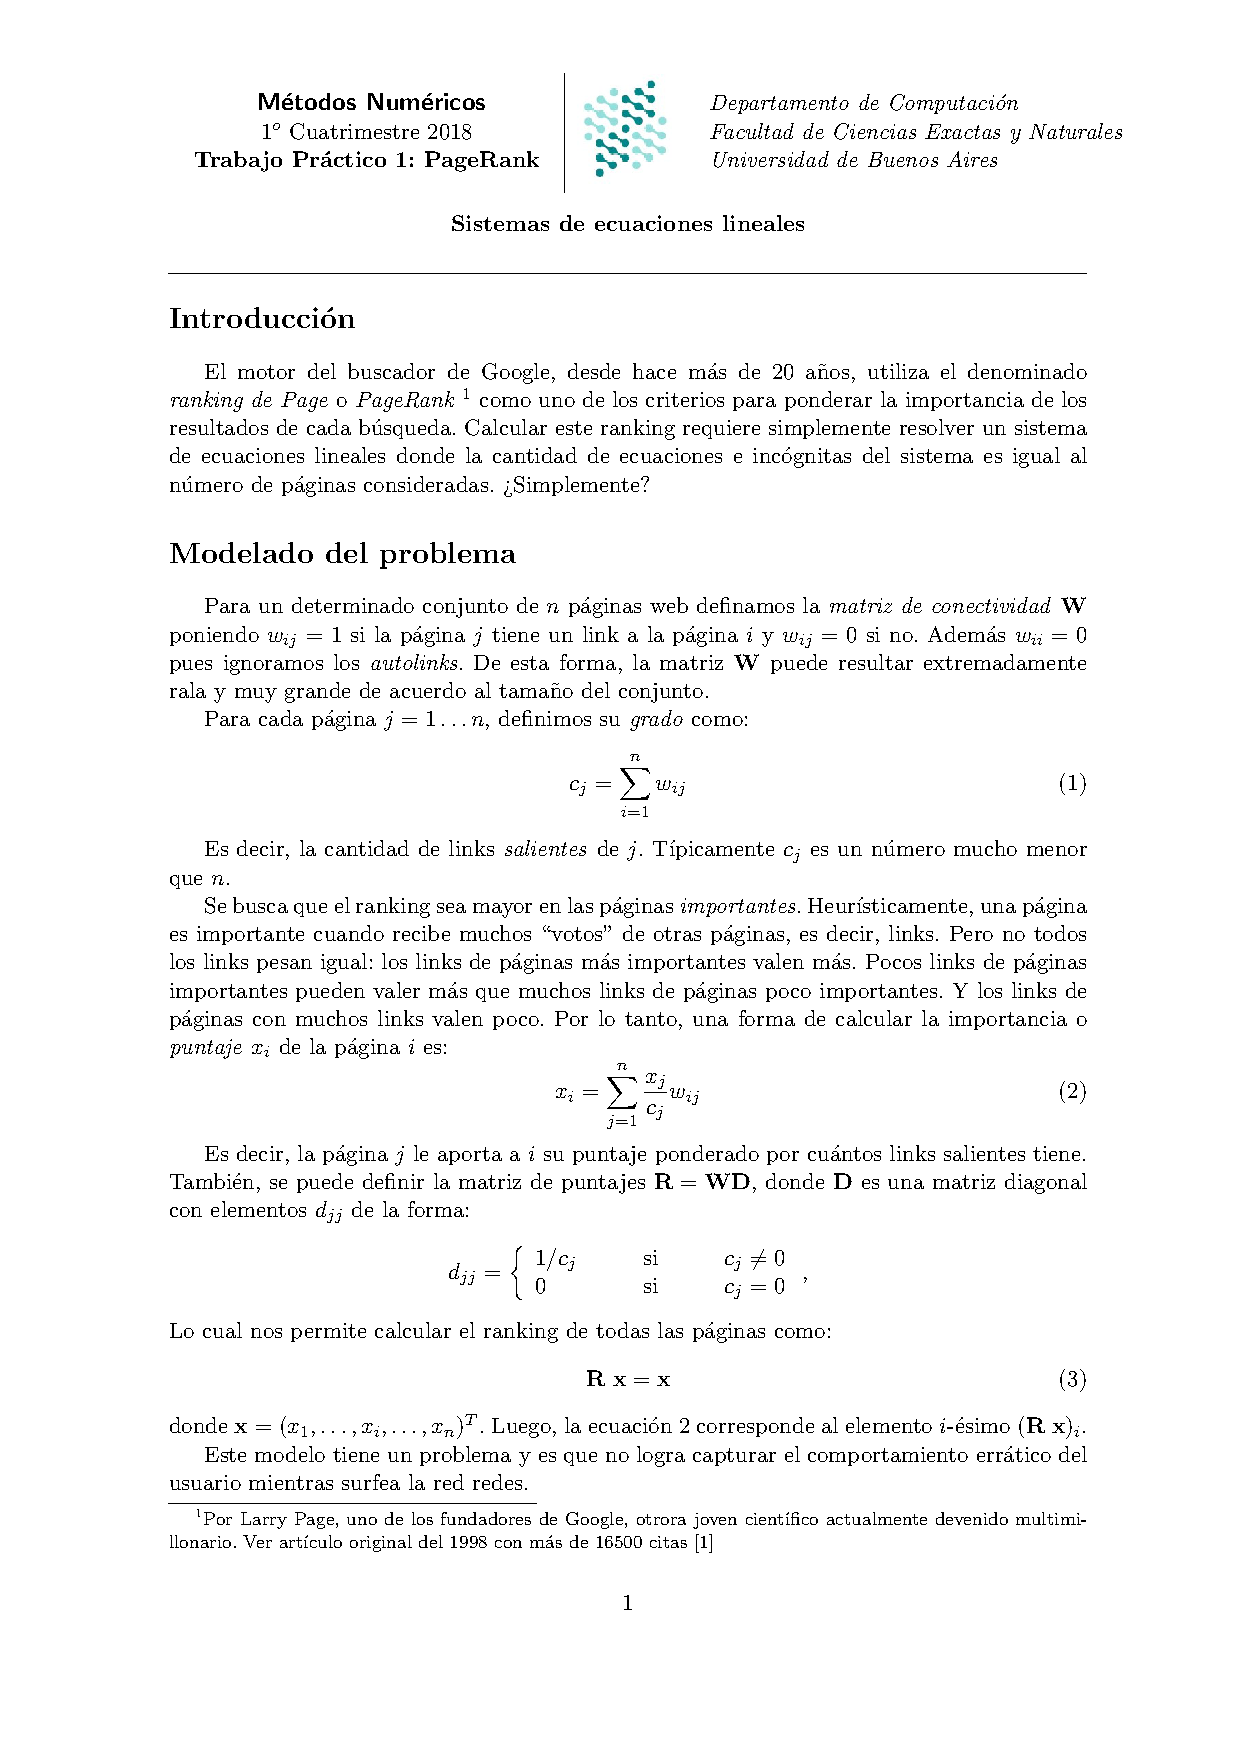
\includepdf[pages=-]{Enunciado.pdf}

